\documentclass[11pt]{article}

\usepackage[margin=1in]{geometry}
\usepackage{amsmath, amssymb}
\usepackage{graphicx}
\usepackage{tikz}
\usepackage{pgfplots}
\usepackage{hyperref}
\usepackage{cite}
\pgfplotsset{compat=1.18}

\title{The Dark Energy Principle: A Falsifiable Reinterpretation of Relativity’s Invariant}
\author{
Luthfi Muslihat \\ 
Independent Researcher \\
\texttt{luthfi.muslihat1@gmail.com} \\
ORCID: \href{https://orcid.org/0009-0001-7428-3600}{0009-0001-7428-3600}
}
\date{November 16, 2025}

\begin{document}
\maketitle

\begin{abstract}
Einstein’s relativity enshrined the speed of light, $c$, as the universal invariant. 
We propose instead that the invariant is the speed of dark energy, $c_{DE}$. 
Photons are contingent travelers whose effective speed depends on cosmic environment. 
This principle predicts achromatic travel-time delays $\Delta t$ that scale with path length $L$ and mean offset $\mu$, producing millisecond to hour-scale lags across voids, filaments, and clusters. 
The framework preserves Lorentz symmetry while offering clean falsification via fast radio bursts (FRBs), gamma-ray bursts (GRBs), and strong lensing time delays.
\end{abstract}

\section{Introduction}
Einstein’s 1905 postulate that the speed of light is invariant for all observers \cite{einstein1905} has shaped modern physics. 
From the Michelson–Morley experiment to GPS synchronization, $c$ has been treated as the ruler of spacetime. 
Yet photons are not isolated; they traverse cosmic structures. 
This raises a provocative question: what if photons are contingent messengers, not the universal invariant?

Dark energy, responsible for cosmic acceleration \cite{frieman2008darkenergy}, permeates spacetime. 
We propose that its characteristic speed, $c_{DE}$, defines the true causal cone. 
Photons, slowed or sped by environment-dependent indices, fall inside this cone, producing achromatic delays.

\section{The Principle}
Let $n_\gamma(x)$ denote the environment-dependent index along a path of length $L$. 
The effective photon speed is
\begin{equation}
c_\gamma(x) = \frac{c_{DE}}{n_\gamma(x)}
\end{equation}
The achromatic delay relative to the $c_{DE}$ baseline is
\begin{equation}
\Delta t = \int_{0}^{L} \frac{dx}{c_\gamma(x)} - \frac{L}{c_{DE}}
= \frac{L}{c_{DE}} \langle n_\gamma - 1 \rangle
= \frac{L}{c_{DE}} \mu
\end{equation}

\section{Geometry of the Cone}
The spacetime interval with $c_{DE}$ defines the true causal cone via $ds^{2} = 0$. 
In units where $c_{DE} = 1$, the cone is traced by $x = \pm t$. 
Photon trajectories satisfy
\begin{equation}
x = \pm c_\gamma t = \pm \frac{t}{n_\gamma}
\end{equation}
placing them inside the true cone when $n_\gamma > 1$. 
The geometric separation encodes the achromatic delay.

\section{Implications}
Replacing $c$ with $c_{DE}$ in Lorentz transformations preserves symmetry:
\begin{equation}
t' = \gamma_{DE}\left(t - \frac{vx}{c_{DE}^{2}}\right), \quad
x' = \gamma_{DE}(x - vt)
\end{equation}
with
\begin{equation}
\gamma_{DE} = \frac{1}{\sqrt{1 - \frac{v^{2}}{c_{DE}^{2}}}}
\end{equation}

\section{Falsifiability}
The principle is falsifiable via:
\begin{itemize}
\item \textbf{Void baseline:} $\Delta t \approx 0$ ms across void sightlines.
\item \textbf{Shuffle collapse:} Randomizing structure abolishes delays.
\item \textbf{Ablation:} DE-only + DM-only contributions approximate full delay.
\item \textbf{Scaling:} $\Delta t \propto L$ and $\Delta t \propto \mu$.
\end{itemize}

\section*{Data Availability}
All simulation notebooks and figures supporting this work are openly available at:  
\url{https://github.com/bynd-id/dark-energy-principle}

\appendix
\section{Formalism}
We formalize the principle by deriving the achromatic delay from first principles.  
Consider a photon traversing a structured environment with index $n_\gamma(x)$.  
The travel time is
\begin{equation}
t_\gamma = \int_{0}^{L} \frac{dx}{c_\gamma(x)} = \frac{1}{c_{DE}} \int_{0}^{L} n_\gamma(x)\, dx
\end{equation}
Relative to the invariant baseline $t_{DE} = L/c_{DE}$, the delay is
\begin{equation}
\Delta t = t_\gamma - t_{DE} = \frac{1}{c_{DE}} \int_{0}^{L} \big(n_\gamma(x) - 1\big)\, dx
\end{equation}
Defining $\mu = \langle n_\gamma - 1 \rangle$, we recover
\begin{equation}
\Delta t = \frac{L}{c_{DE}} \mu
\end{equation}

\section{Figures}
\begin{figure}[h]
\centering
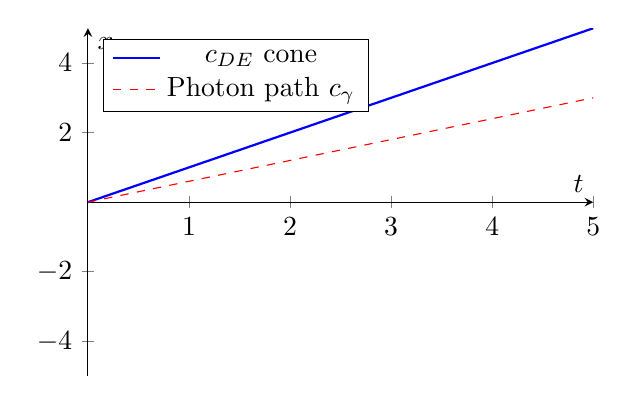
\begin{tikzpicture}
\begin{axis}[
    axis lines = middle,
    xlabel = {$t$},
    ylabel = {$x$},
    width=8cm,
    height=6cm,
    xmin=0, xmax=5,
    ymin=-5, ymax=5,
    legend pos=north west
]
\addplot[blue, thick] coordinates {(0,0) (5,5)};
\addlegendentry{$c_{DE}$ cone}
\addplot[red, dashed] coordinates {(0,0) (5,3)};
\addlegendentry{Photon path $c_\gamma$}
\end{axis}
\end{tikzpicture}
\caption{True causal cone defined by $c_{DE}$ (blue) and contingent photon path $c_\gamma$ (red).}
\end{figure}

\begin{figure}[h]
\centering
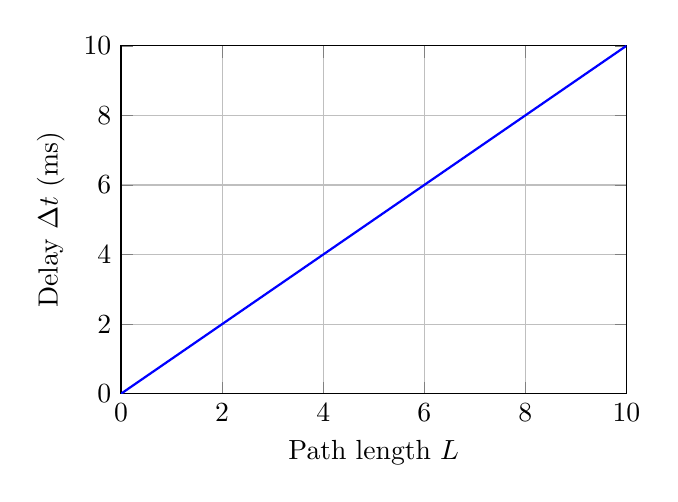
\begin{tikzpicture}
\begin{axis}[
    xlabel={Path length $L$},
    ylabel={Delay $\Delta t$ (ms)},
    width=8cm,
    height=6cm,
    xmin=0, xmax=10,
    ymin=0, ymax=10,
    grid=major
]
\addplot[blue, thick] coordinates {(0,0) (2,2) (4,4) (6,6) (8,8) (10,10)};
\end{axis}
\end{tikzpicture}
\caption{Linear scaling of achromatic delay $\Delta t$ with path length $L$.}
\end{figure}

\bibliographystyle{unsrt}
\begin{thebibliography}{99}
\bibitem{einstein1905} A. Einstein, ``On the Electrodynamics of Moving Bodies,'' Annalen der Physik, 1905. doi:10.1002/andp.19053221004
\bibitem{frieman2008darkenergy} J. Frieman, M. Turner, D. Huterer, ``Dark Energy and the Accelerating Universe,'' Annual Review of Astronomy and Astrophysics, 2008. doi:10.1146/annurev.astro.46.060407.145243
\bibitem{frbCosmoArxiv} Z.-W. Zhao et al., ``Probing dark energy with FRBs,'' arXiv:2210.07162
\bibitem{treu2022lensing} T. Treu, S. Suyu, P. Marshall, ``Strong lensing time-delay cosmography,'' A\&A Review, 2022. doi:10.1007/s00159-022-00139-y
\end{thebibliography}

\end{document}